\chapter{Funnels}

The term \funnel\ first appears in \cite{masonMechanicsManipulation1985}. The
\funnel\ definitions in this thesis is taken from a series of articles on
\funnel 's \cite{tobenkinInvariantFunnelsTrajectories2010}
\cite{tedrakeLQRtreesFeedbackMotion2009} \cite{majumdarRobustOnlineMotion2013}
\cite{majumdarFunnelLibrariesRealtime2017}
\cite{ahmadiDSOSSDSOSOptimization2017}, with the main focus being on
\cite{majumdarFunnelLibrariesRealtime2017}. Here a \funnel\ is mathematically
defined as
\[
  \bar{x}(0) \in \mathcal{X}_0 \Rightarrow \bar{x}(t) \in F(t), \forall t \in
  \sqb{0,T}
\]
where \(\mathcal{X}_0\) is the set of initial conditions, \(\sqb{0,T}\) the time
interval, and \(F(t)\) is the set of states that the system can be in at time
\(t\). Although this thesis concerns itself with approximating the reachable set
through \textit{Lyapunov} functions. A useful analogy is imagining the funnel
created through a \textit{Monte-Carlo} simulation, where the \funnel would be
the set of all the paths traversed by the dynamical system at hand. For a simple
car model, this could look similar to:

\begin{figure}
  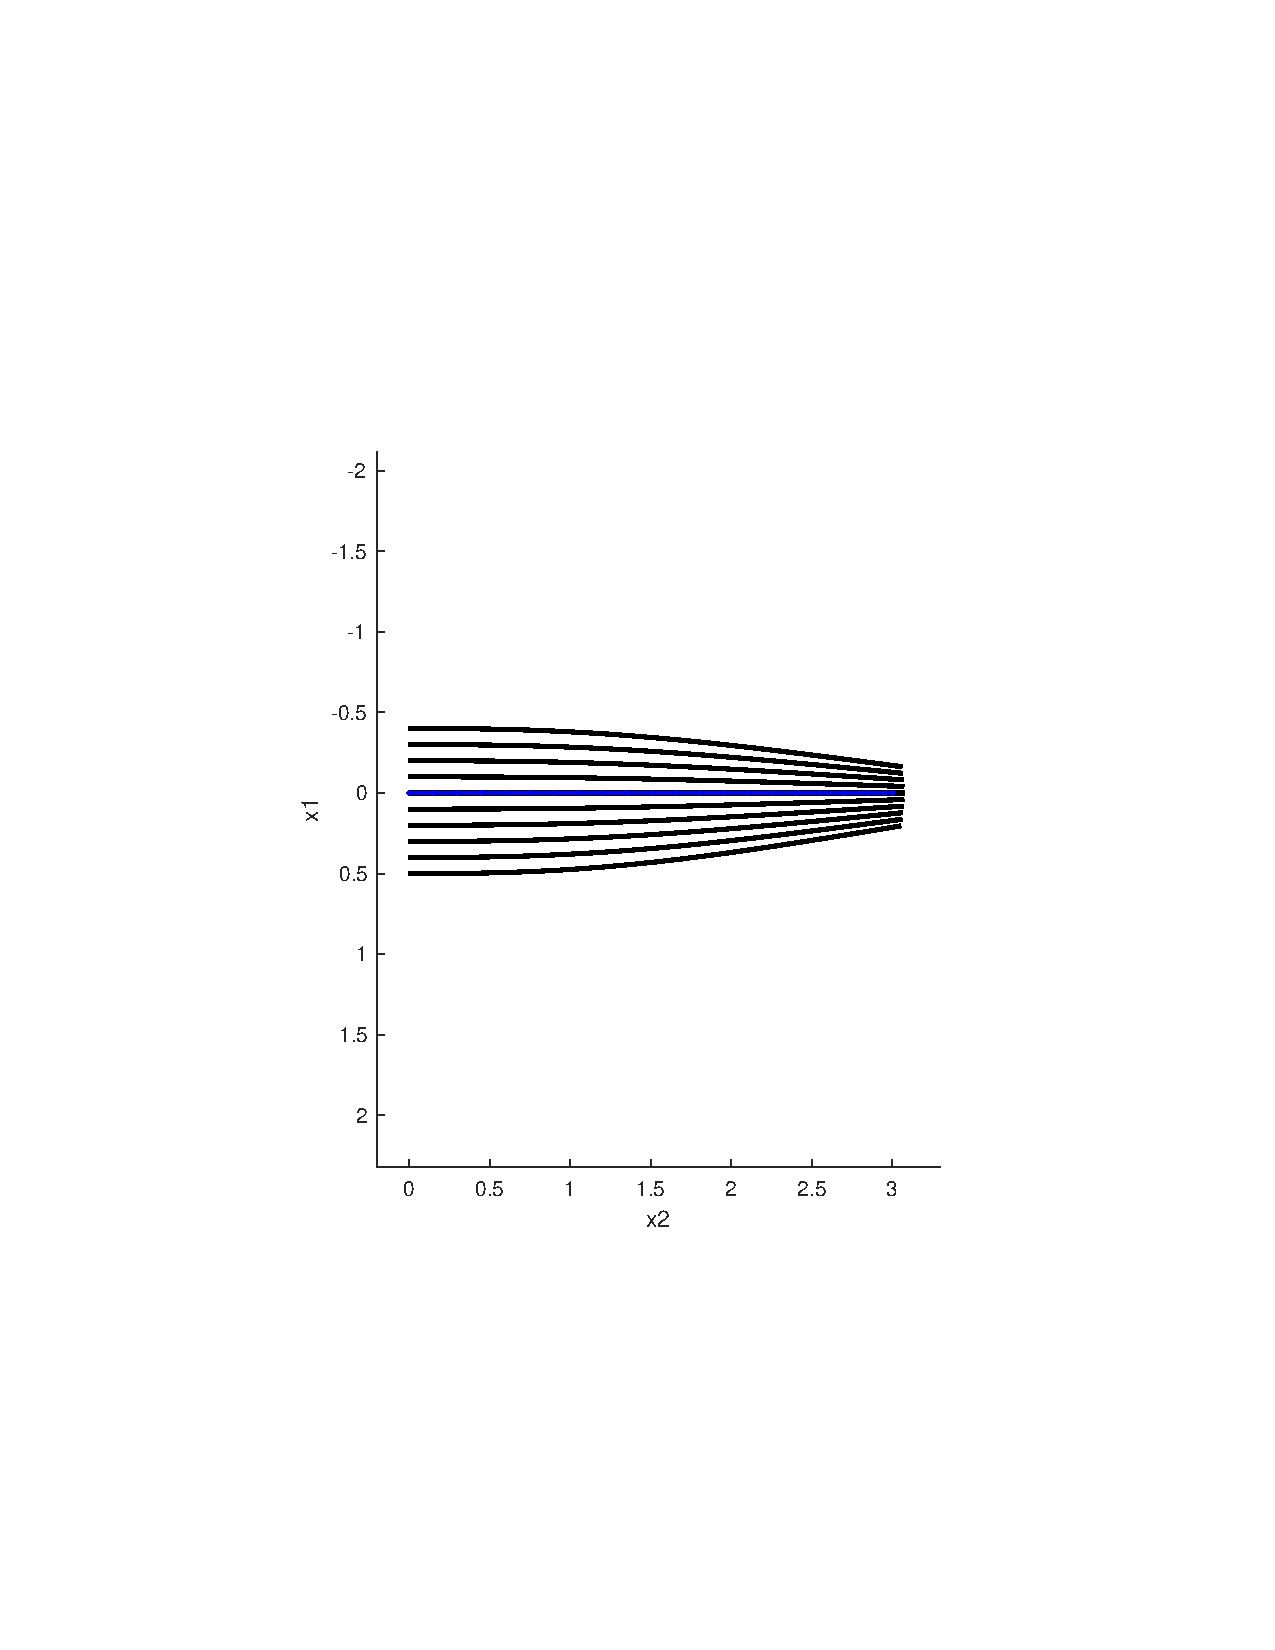
\includegraphics[scale=.5]{figures/funnels/montecarlofunnel}
  \caption{The simulation of N paths starting from a random point in the
    interval \(\sqb{-1,1}\), and controlled with a LQR controller.}
\end{figure}

\subsection{Lyapunov Functions}

A \textit{Lyapunov function} for an autonomous dynamical system is defined as a
scalar function \(V: \R^n \rightarrow \R\), with continuous first derivatives,
is locally positive definite, and \(\Delta V \dot g\) is also locally negative
definite. The \textit{Lyapunov functions} can then be used to prove the
\textit{Lyapunov stability} of the dynamical system. if \(\dot{x} = f(x)\) is a
dynamical system, and \(\dot{V}\) is the time derivate of the
\textit{Lyapunov-candidate function} \(V\), then:
\[
  \dot{V}(x) = \frac{d}{dt}V(x(t)) = \frac{\partial V}{\partial x} \cdot
  \frac{dx}{dt} = \Delta V \cdot \dot{x} = \Delta \cdot f(x)
\]

\subsection{Lyapunov Stability}

A function being stable in the sense of \textit{Lyapunov}, is defined as: Given
the autonomous nonlinear dynamical system
\[
  \dot{x} = f(x(t)), \, x(0) = x_0
\]
with \(\x(t)\) denotes the state vector of the system, with \(x(t) \in
\mathcal{D} \subseteq \R^n\). \(\mathcal{D}\) is an open set containing the
origin, and \(f \colon \mathcal{D} \rightarrow \R^n\) continous on
\(\mathcal{D}\). Suppose that \(f\) has an equilibrium at \(x_e\) so that
\(f(x_e) = 0\), then this equilibrium is \textit{Lyapunov stable} if for every
\(\epsilon > 0\) there exists a \(\delta > 0\) such that if \(\left \lVert x(0)
  - x_e \right \rVert < \delta\) then for every \(t \geq 0\) we have \( \left
  \lVert x(t) - x_e \right \rVert \leq \epsilon\).

Conceptually this means that a solution starting out in the vincinity of the
equilibrium (\(\delta\)), will remain close (\(\epsilon\)) to it. Also note that
this must be true for any \(\epsilon\) one may choose. (semicite wikipedia?).

\subsection{Lyapunov's second method for stability}

\textit{Lyapunov's} second method (also referred to as \textit{Lyapunov's}
direct method) for stability makes use of the \textit{Lyapunov} function \(V\).
If given a dynamical system of the form \(\dot{x} = f(x)\) having a point of
equilibrium at \(x = 0\). Consider a function \(V(x) \colon \R^n \rightarrow
\R\), such that
\begin{align*}
  V(x) &= 0 \text{ if and only if } x = 0 \\
  V(x) &> 0 \text{if and only if} x \neq 0 \\
  \dot{V}(x) &= \frac{d}{dt}V(x) = \sum_{i=0}^{n} \frac{\partial V}{\partial x_i} f_i(x) \leq 0 \text{ for all values of } x \neq 0. \\
\end{align*}
Then \(V(x)\) is called a \textit{Lyapunov function} candidate and the system is
stable in the sense of Lyapunov. (semicite wikipedia).

The following sections \ref{subsec:LaSalle's invariance
  principle},\ref{subsec:LaSalle's invariance principle},\ref{subsec:Lyapunov
  analysis for linear systems}, are based on the lecture notes from
\cite{tedrakeUnderactuatedRoboticsAlgorithms2019}, and are adapted slightly for
presentation in this thesis.

\subsection{LaSalle's invariance principle}
\label{subsec:LaSalle's invariance principle}

\textit{LaSalle}'s invariance principle formalizes the convergence of a
dynamical system to an invariant set, rather than to a fixed point. Defined as:
Given a system \(\dot{x} = f(x)\) with \(f\) continuous. If we produce a scalar
function \(V(x)\) with continous derivatives for which over an open subset
\(\mathcal{B} \in \R^n\) we have
\begin{align*}
  V(x) \geq 0, \; \dot{V}(x) \leq 0,
\end{align*}
and \(V(x) \rightarrow \infty\) as \(\norm{x} \rightarrow \infty\), then \(x\)
will converge to the largest \textit{invariant set} where \(\dot{V}(x) = 0\).
Where an \textit{invariant set}, \(\mathcal{G}\), of the dynamical system is a
set for which \(x(0) \in \mathcal{G} \Rightarrow \forall t > 0,\, x(t) \in
\mathcal{G}\). Meaning that once you enter the region of invariance, you never
leave; which will be important for our funnel calculations later on.

\subsection{Lyapunov analysis with convex optimization}
\label{subsec:Lyapunov analysis with convex optimization}

One of the primary limitations in Lyapunov analysis is that it is potentially
very difficult to come up with suitable \textit{Lyapunov} function candidates
for underactuated systems. Even if given a \textit{Lyapunov} function, simply
checking that the \textit{Lyapunov} conditions hold for all \(x\) can be
difficult. Imagine checking that \(\dot{V}\) is strictly negative for all \(x\),
except at the origin, if \(\dot{V}\) is some complicated nonlinear function over
a vector \(x\). However with recent advances in convex optimization
\cite{parilloStructuredSemidefinitePrograms}, there now exists the opportunity
to numerically search for these functions.

A natural approach to a numerical algorithm for verifying \textit{Lyapunov}
stability could be to evaluate \(V\) and \(\dot{V}\) at a large number of points
and check that \(V\) is positive, and that \(\dot{V}\) is negative. Which
\href{https://github.com/RobotLocomotion/drake/blob/master/systems/analysis/test/lyapunov_test.cc}{does
  in fact work}. But in reality we can do better, using optimization algorithms
which rigourously checks these conditions \textit{for all \(x\)}, without the
need for dense sampling. Which in actuality enables us to search for
\textit{Lyapunov functions} in an infinite function space (which is what makes
up the space of all \textit{Lyapunov} functions).

\subsection{Lyapunov analysis for linear systems}
\label{subsec:Lyapunov analysis for linear systems}

\begin{theorem}
  Given a linear system of the form \(\dot{x} = Ax\) if one can find a
  \textit{Lyapunov function}
  \[
    V(x) = x^TPx, \; P = P^T \succeq 0
  \]
  which also satisfies
  \[
    \dot{V} = x^TPAx + x^TA^TPx \succeq 0.
  \]
  Then the origin is globally asymptotically stable.
\end{theorem} \cite{tedrakeUnderactuatedRoboticsAlgorithms2019}

For the linear case the existence of a quadratic \textit{Lyapunov} function is a
necesary and sufficient condition. Furthermore, a \textit{Lyapunov} function can
always be found by finding the positive definite solution to the matrix Lyapunov
equation
\[
  PA + A^TP = -Q
\]
for any \(Q = Q^T \geqslant 0\).

\subsection{The connection between Lyapunov analysis and convex optimization}

The first connection between Lyapunov analysis and convex optimization will be a
\ac{SDP}-program. In fact the Lyapunov conditions for a linear system can be
formulated in the form of an \ac{SDP} - which is a form of convex optimization.
For any problem formulated as an \ac{SDP} there exists an efficient - and
optimal - solution, barring numerical difficulties.

\subsection{Numerical convex optimization}

\subsubsection{Linear programming}

\subsubsection{Semidefinite programming}

A wide variety of nonlinear convex optimization problems can be formulated and
efficiently solved as \ac{SDP}s. In control theory, semidefinite programming is
a method for numerically finding the optimal solution of a linear matrix
inequality. It is concerned with the optimization of a linear objective function
over the intersection of the \textit{cone} of positive semidefinite matrices
with an affine space.

A convex cone is a subset of a vector space over an ordered field that is closed
under linear combinations with positive coefficients.

\begin{figure}
  \includegraphics[scale=.5]{figures/funnel/Convex_cone_illust}
  \caption{A convex cone (light blue). Inside of it, the light red convex cone
    consists of all points \(\alpha x + \beta y \) with \(\alpha,\, \beta > 0\),
    for the depicted \(x\) and \(y\). The curves on the upper right symbolize
    that the regions are infinite in extent.
    \cite{alexandrovConvexConeIllust2019}}
\end{figure}

A semidefinite program can solve all problems of the form:
\begin{align*}
  \text{minimize } &TrCX \\
  \text{subject to } &TrA_iX = b_i \text{for all i } = 1,\ldots,m\\
                   &X \succeq 0
\end{align*} 
where \(X \in S^n\), with \(S^n\) being the space of real symmetric \(nxn\)
matrices. The vector \(b \in \R^m\), and the matrices \(A_i \in S^n\), and \(C
\in S^n\) are given problem
parameters\cite{wolkowiczHandbookSemidefiniteProgramming2000}.

\subsection{A simple example}
\label{subsec:A simple example}

\begin{align*}
  \text{min(a), subject to}
  \begin{bmatrix}
    a & 0 \\
    0 & 1 \\
  \end{bmatrix}
  \succeq 0
\end{align*}\cite{tedrakeUnderactuatedRoboticsAlgorithms2019}

The linear Lyapunov example from above \ref{subsec:Lyapunov analysis for linear
  systems}, can also be formulated as an \ac{SDP} like so:
\begin{align*}
  \text{find p, subject to } P \succeq 0, \; PA + A^TP \preceq 0.
\end{align*}\cite{tedrakeUnderactuatedRoboticsAlgorithms2019}

This formulation then provides the ground for an automatic search for a
\ac{LQR}-controller. Shown below, is also how one can make it robust to bounded
uncertainties.

Given the system \(\dot{x} = Ax\), where \(A\) is unknown, with bounded
uncertain parameters. This set can be described by writing \(A\) as an uncertain
linear combination of known matrices, e.g:
\[
  A = \sum_{i} \beta_{i}A_{i}, \; \sum_{i}\beta_{i} = 1, \; \forall i,\beta_{i}
  > 0
\]
Geometricall the formulation descibes a polygon in the \(A\) space, with each
vertice being one of the \(A_{i}\) which is used to describe a as a linear
combination.

\begin{figure}
  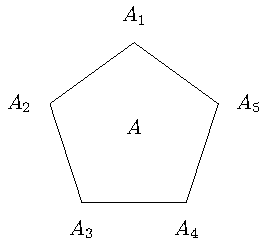
\includegraphics{figures/funnel/linearuncertainlyapunov}
  \caption{Illustration of the search space. Adapted from
    \cite{tedrakeUnderactuatedRoboticsAlgorithms2019}}
\end{figure}

This problem, once formulated can the be sent to an automatic \ac{SDP}-solver,
such as \textit{MOSEK}\cite{mosek}, which is used in this thesis.

This example is important as it provides a way in which to search an infinite
function space (The Lyapunov functions) - numerically - for a function which
fullfills our constraints, and solves the problem. Furthermore, the solution is
optimal as long as the problem is convex. Downside, however, is that this method
only works on linear systems, and the problem at hand in this thesis is
nonlinear.

Fortunately, with the advent of \ac{SOS} programming, it is now possible to
formulate the search for Lyapunov functions as a convex optimization problem.

\section{SOS}

The tools to search for a Lyapunov function for a nonlinear system relies on the
algebraic geometry theory of \ac{SOS}, which is about representing
\textit{non-negative polynomials} as a sum of squares of polynomials. In short,
if one can write a polynomial \(p\) with indeterminates \(x_1,x_2,\ldots,x_n\)
is \ac{SOS} if
\[
  p(x) = \sum_{i=1}^{m}g_i^2(x)
\]
for \(g_i \in \P\), where \(\P\) is the space of polynomials. The clue here is
that every form that is \ac{SOS} is also a positive polynomial, although the
converse is not necessarily true\cite{majumdarFunnelLibrariesRealTime2016}.

This is an important detail, as the numerical search for Lyapunov functions can
only verify \ac{SOS}-polynomials, and as such there will be a \textit{gap} in
the Lyapunov functions we can find and verify, and the best Lyapunov functions
for the task, as it is no guarantees that a \ac{SOS}-Lyapunov function will be
the optimal function for the task.

\ac{SOS} is the theory of

As seen in section \ref{subsec:A simple example}, if one is able to

\acl{SOS} polynomials are

\acl{SOS} programming is

\cite{parilloStructuredSemidefinitePrograms},

\subsection{SOS programming}

The procedure used for searching the space of all positive Lyapunov functions
which can be written as a sum of squares is \ac{SOS} programming. With
\cite[Parillo's]{parilloStructuredSemidefinitePrograms}, work, there now exists
an efficient way of restructuring a \ac{SOS} program into an \ac{SDP} program,
solve it, then convert it back, and get the sought solution polynomial.

\ac{SOS} programming relies on the ability to write a SOS polynomial in the form
\begin{align*}
  p(x) &= s(x)^TQs(x)\\
\end{align*}
where \(p(x)\) is a \ac{SOS} polynomial, and \(Q\) is \ac{PSD}, and \(s(x)\) is
a vector of \textit{monomials} - meaning that its elements are the terms in a
polynomial, like so
\[
  s(x) = \begin{bmatrix} 1 \\ x \\ y \\ x^2 \\ xy \\ y^2 \end{bmatrix}
\]
where \(s(x)\) is a monomial in \(x\) and \(y\) of order two.In general \(s(x)\)
is a monomial with degree less than or equal to half that of
\(p(x)\)\cite{parilloStructuredSemidefinitePrograms}\label{monomialdegree}. The condition that
\(s(x)\) is \ac{SOS} is much more \textit{computationally tractable} than a
nonnegativity constraint \cite{parilloStructuredSemidefinitePrograms}. The
methodology used in the \ac{SOS} program in this thesis is based on the
relaxation from \cite{parilloStructuredSemidefinitePrograms}, which in turn is
based on the \textit{Positivstellensatz} from algebraic geometry. In this type
of problem the interest is in finding polynomials \(p_i(x), \,
i=1,2,\ldots,\hat{N}\), and sums of squares \(p_i(x), \,
i=(\hat{N}+1),\ldots,N\), such that
\[
  a_{0,j}(x) + \sum_{i=1}^{N}p_{i}(x)a_{i,j}(x) = 0, \; \text{for } j =
  1,2,\ldots,J.
\]
where \(a_{i,j}(x)\) are given constant coefficient polynomials. Problems of
this type is what will be referred to as \ac{SOS} programs throughout this
thesis\cite{sostools}. Without going into more details here in the
preliminaries, the advantage of \ac{SOS} programming is that it enables the
solution of problems which can be formulated having positivity constraints of
the kind \(f(x) \geq 0\).

\subsubsection{A simple example}

\[
  p = 2 - 8x + 17x^2
\]
which is a sum of squares polynomial, as it can be written in the form
\[
  p = \sum_{i=1}^{N}g_i^2(x) = g_1^2(x) + g_2^2(x) + g_3^2(x)= 1 + (1-4x)^2 + x^2
\]
which shows that \(p(x)\) is positive for all x. In fact, \(p\) is \ac{SOS} if and only
if there exists a \acl{PSD} matrix \(Q\), such that \(p(x) = s(x)^TQs(x)\).
Also, the problem can be formulated using \textit{monomials} of degree one
(square root of the degree of \(p\))\ref{monomialdegree}.

From now on, a constraint of the form \(f(x) \geq 0,\, \forall x\) will be written as \(f(x)
\in SOS\).

\subsection{Lyapunov analysis using SOS programming}

With the link shown between positive polynomials and \ac{SOS} programming, it is
time to start looking at the link between Lyapunov functions and SOS
programming. Thus, given a dynamical system of the form \(\dot{x} = f(x)\), and
a Lyapunov function of the form
\[
  V(x) = \sum_{i=0}^d a_ix_i
\]
with \(d\) being the degree of the polynomial, a \ac{SOS} program
\begin{align*}
  \text{find \(\alpha\)}&, \text{ subject to } V(x) \text{ is SOS}\\
  -\dot{V}(x) &= -\frac{\partial V}{\partial x}f(x) \text{ is SOS}.\\
\end{align*}
\cite{tedrakeUnderactuatedRoboticsAlgorithms2019}
and because this is a convex optimization problem, the solver will return a
solution if one exists.

\subsubsection{Example - The damped simple pendulum}

As a simple example where a search for a polynomial Lyapunov function can be
performed is the \textit{simple pendulum} example. The dynamics of the pendulum
can be described as
\[
  ml^2\dot{\dot{\theta}} + mgl sin(\theta) = -b\dot{\theta}
\]
which in vector form can be written as
\begin{align*}
  \dot{\theta}_1 &= \theta_2 \\
  \dot{\theta}_2 &= f(\theta_1,\theta_2) = -\frac{g}{l}sin(\theta_1) -\frac{b}{ml^2}\theta_2
\end{align*}
with \(\theta_1 = \theta\), and \(\theta_2 = \dot{\theta}\).

There is still one problem however. Notice that the equations are not
polynomial, which is required if the \ac{SOS} programming framework is to be
applied. There are in general two ways of dealing with this:

First method, is to Taylor expand equation. Second, is doing a change of
coordinates of the form \(\left[ \theta \; \dot{\theta} \right] \) to \(\left[ s
  \;c \; \dot{\theta} \right]\), where \(s = sin(\theta)\) and \(c =
cos(\theta)\). Then with \(x = \left[ s \; c \; \dot{\theta} \right]^T\) the dynamics
can be written as
\[
  \dot{x} =
  \begin{bmatrix}
    c\dot{\theta} \\
    -s\dot{\theta} \\
    - \frac{1}{ml^2} \left( b\dot{\theta} + mgl s \right)
  \end{bmatrix}
\]

Although this is a nice trick, and could be employed for the vehicle model which
will be used, the code in this thesis will stick with Taylor expansions as it
enables changing the model at hand a lot easier.

Now, parametrizing a Lypunuv candidate function as
\[
  V = \alpha_0 + \alpha_1s + \alpha_2c + \cdots + \alpha_9s^2 + \alpha_{10}sc + \alpha_{11}s\dot{\theta}
\]
and formulating the search for a feasible Lyapunov function
\begin{example}
  find  \(\alpha\) subject to \(V\) is SOS, and \(-\dot{V}\) is SOS
\end{example}

Actually this feasability problem can be reduced further. In fact \(V\) and
\(\dot{V}\) need only be positive in the case that \(sin(\theta)^2 +
cos(\theta)^2 = 1\). This then means that the problem can be formulated as
\begin{align*}
  &\text{find}\alpha \lambda \\
  &\text{subject to } V \text{ is SOS} \\
  &-\dot{V}(x) - \lambda(x)\left( s^2 + c^2 -1 \right) \text{ is SOS}
\end{align*}
which is a standard method for proving nonnegativity of polynomials on
semialgebraic sets (sets described by inequalities) called the
\textit{S-procedure}, which will be the topic of the next section.

\subsection{S-procedure}

The \textit{S-procedure} is used to check for positivity (SoS) over a region.

\subsection{Common Lyapunov functions for uncertain systems}
\subsubsection{Robust set-invariance}

A sub-level set of the Lyapunov function is, in comparison with the system
without uncertainties, not guaranteed that every sub-level set of the Lyapunov
function is not necessarily invariant. (Give example.).



\section{Transformation of funnels}

\subsection{Cyclic coordinates?}

How de we transform the funnels to different angles and coordinates.

\subsection{Non-cyclic coordinates}

\subsection{Adding uncertainty to the funnels}

The funnels can take uncertainty into account. Adding this in accordance with
the paper by \cite{majumedar2013}. For now adding this for dimension (?).

\subsection{Scaling the funnels by the size of the vehicle simulated}

The model used in this thesis is a point model. As so, it is not ready for use
in simulations as is, whereas the vehicle used in the model has some given
length and width. Therefore the Funnel needs to be scaled to handle the given
size of the vehicle. TODO - how to do this proper? Check out the FunnelLibrary.m
file for an example on how to do this proper.

\subsection{Testing the funnels}

After we have generated our Funnels, it is time to test them through a
simulation. We start out by first simulating the Funnels with the uncertain
plant dynamics, and checks if the model ever leaves the verified parametrized
set. From this we get:

\begin{figure}
  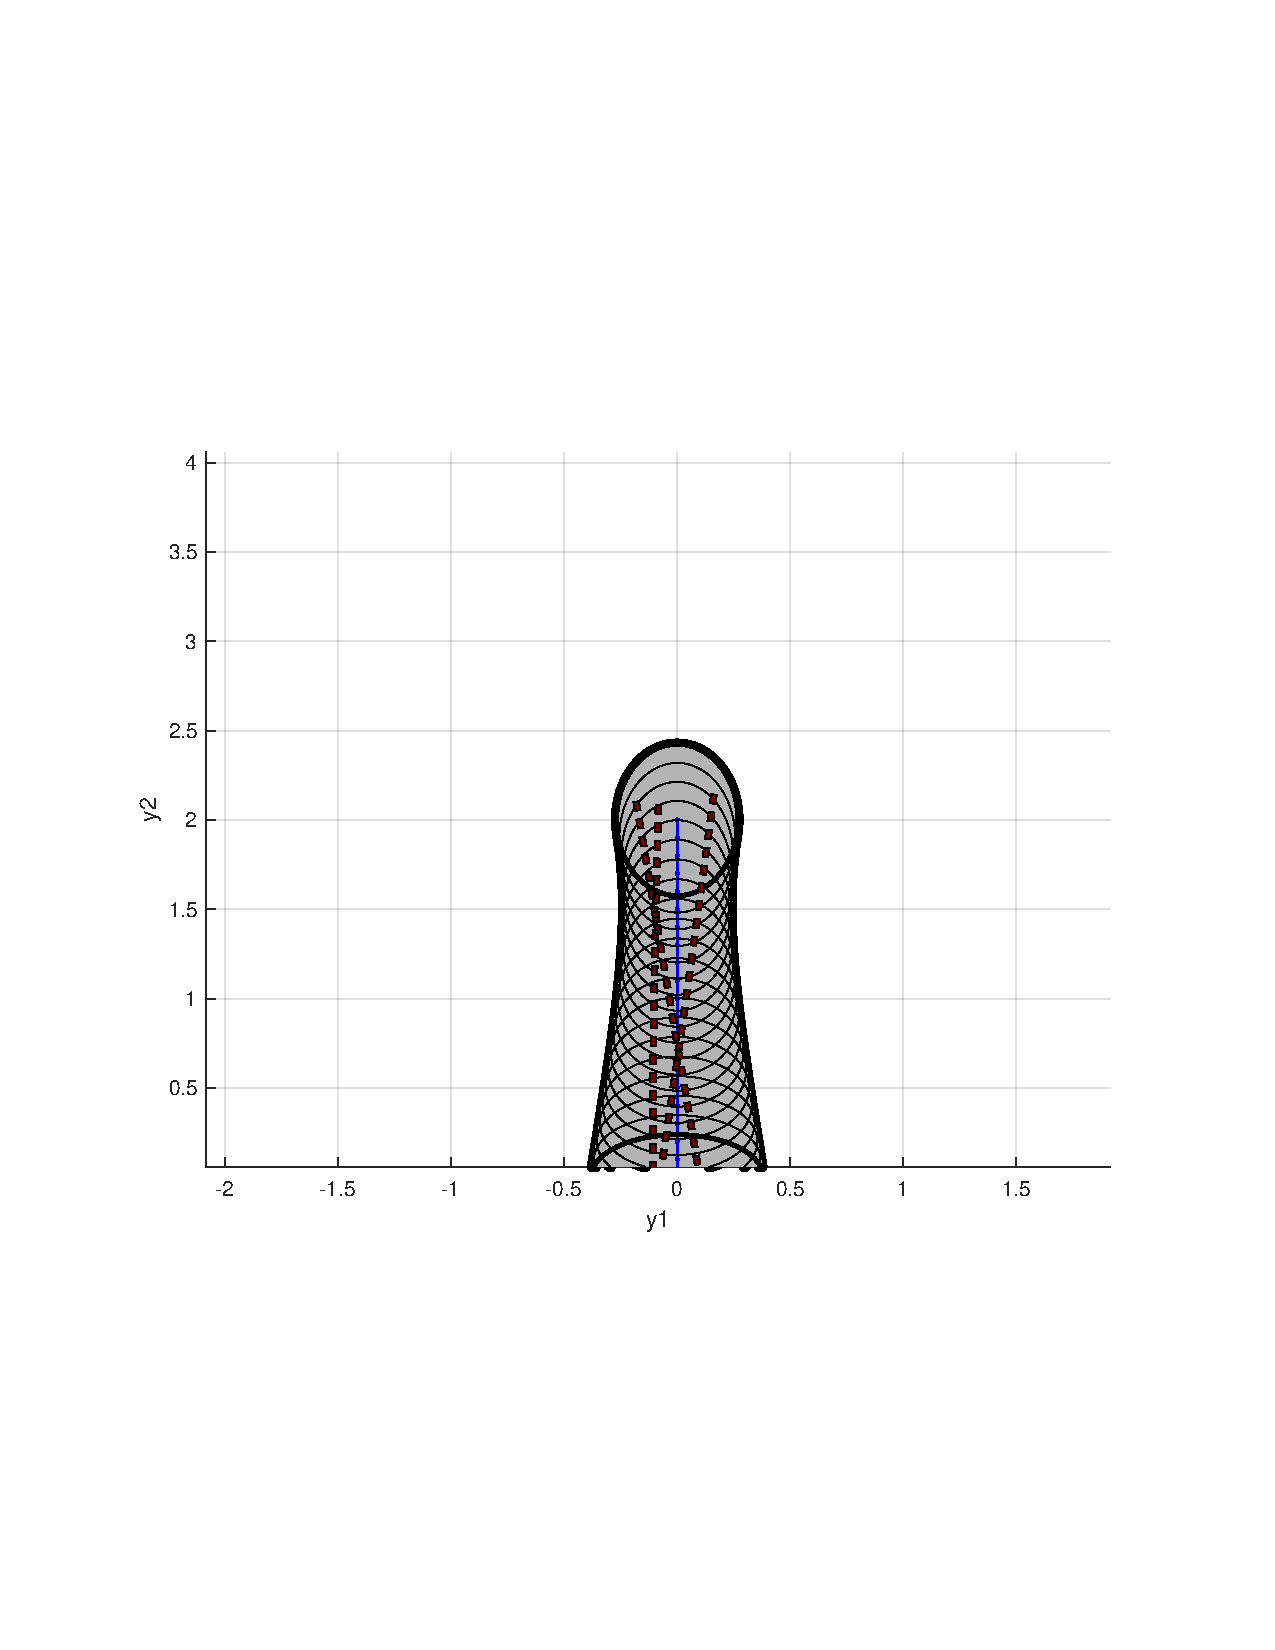
\includegraphics[scale=0.5]{figures/funnel/straight_simulation}
  \caption{Three simulations of the straight funnel with different initial
    conditions, where all three funnels stayed inside the funnel. However, they
    do seem to not converge towards the original trajectory.}
\end{figure}


\begin{figure}
  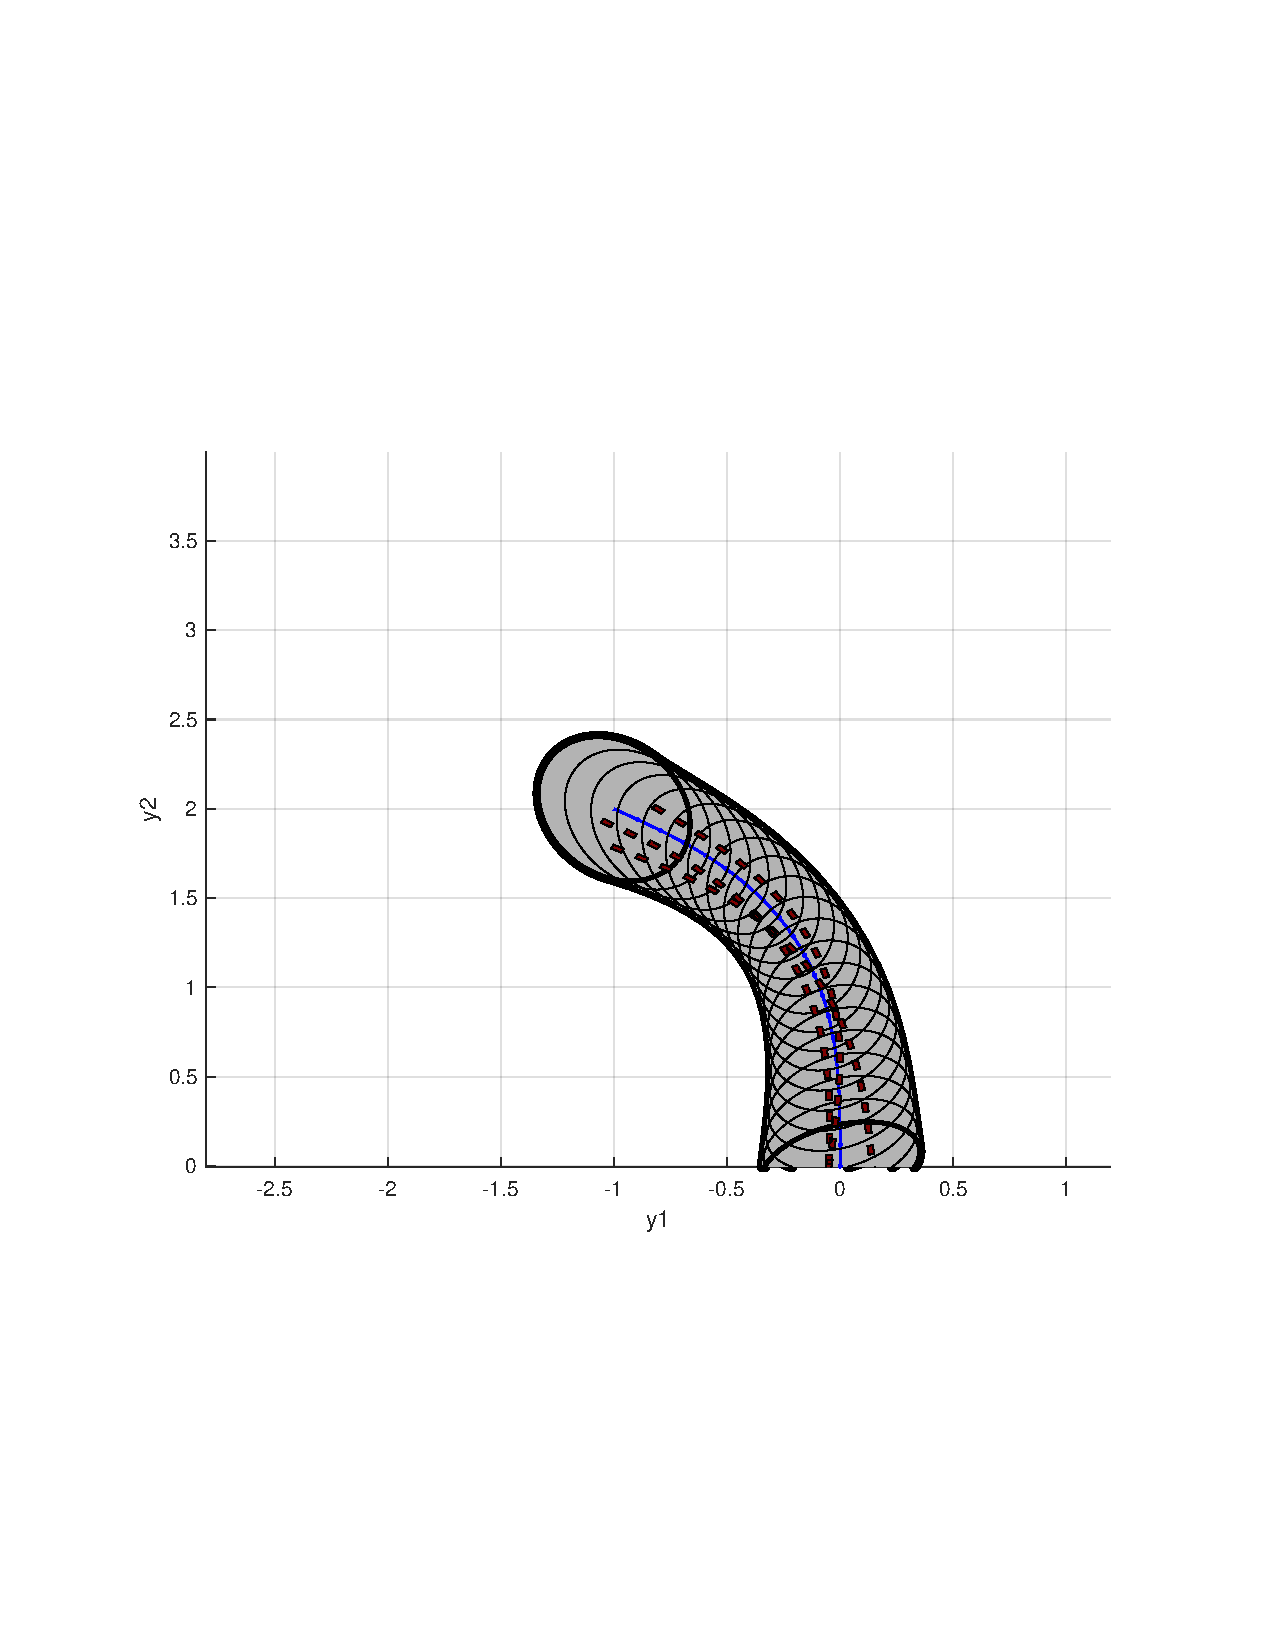
\includegraphics[scale=0.5]{figures/funnel/left_simulation}
  \caption{Three simulations of the left funnel with different initial
    conditions, where two out of three funnels left the inside of the funnel.
    Right now I can only speculate as to why this is happening.}
\end{figure}


\begin{figure}
  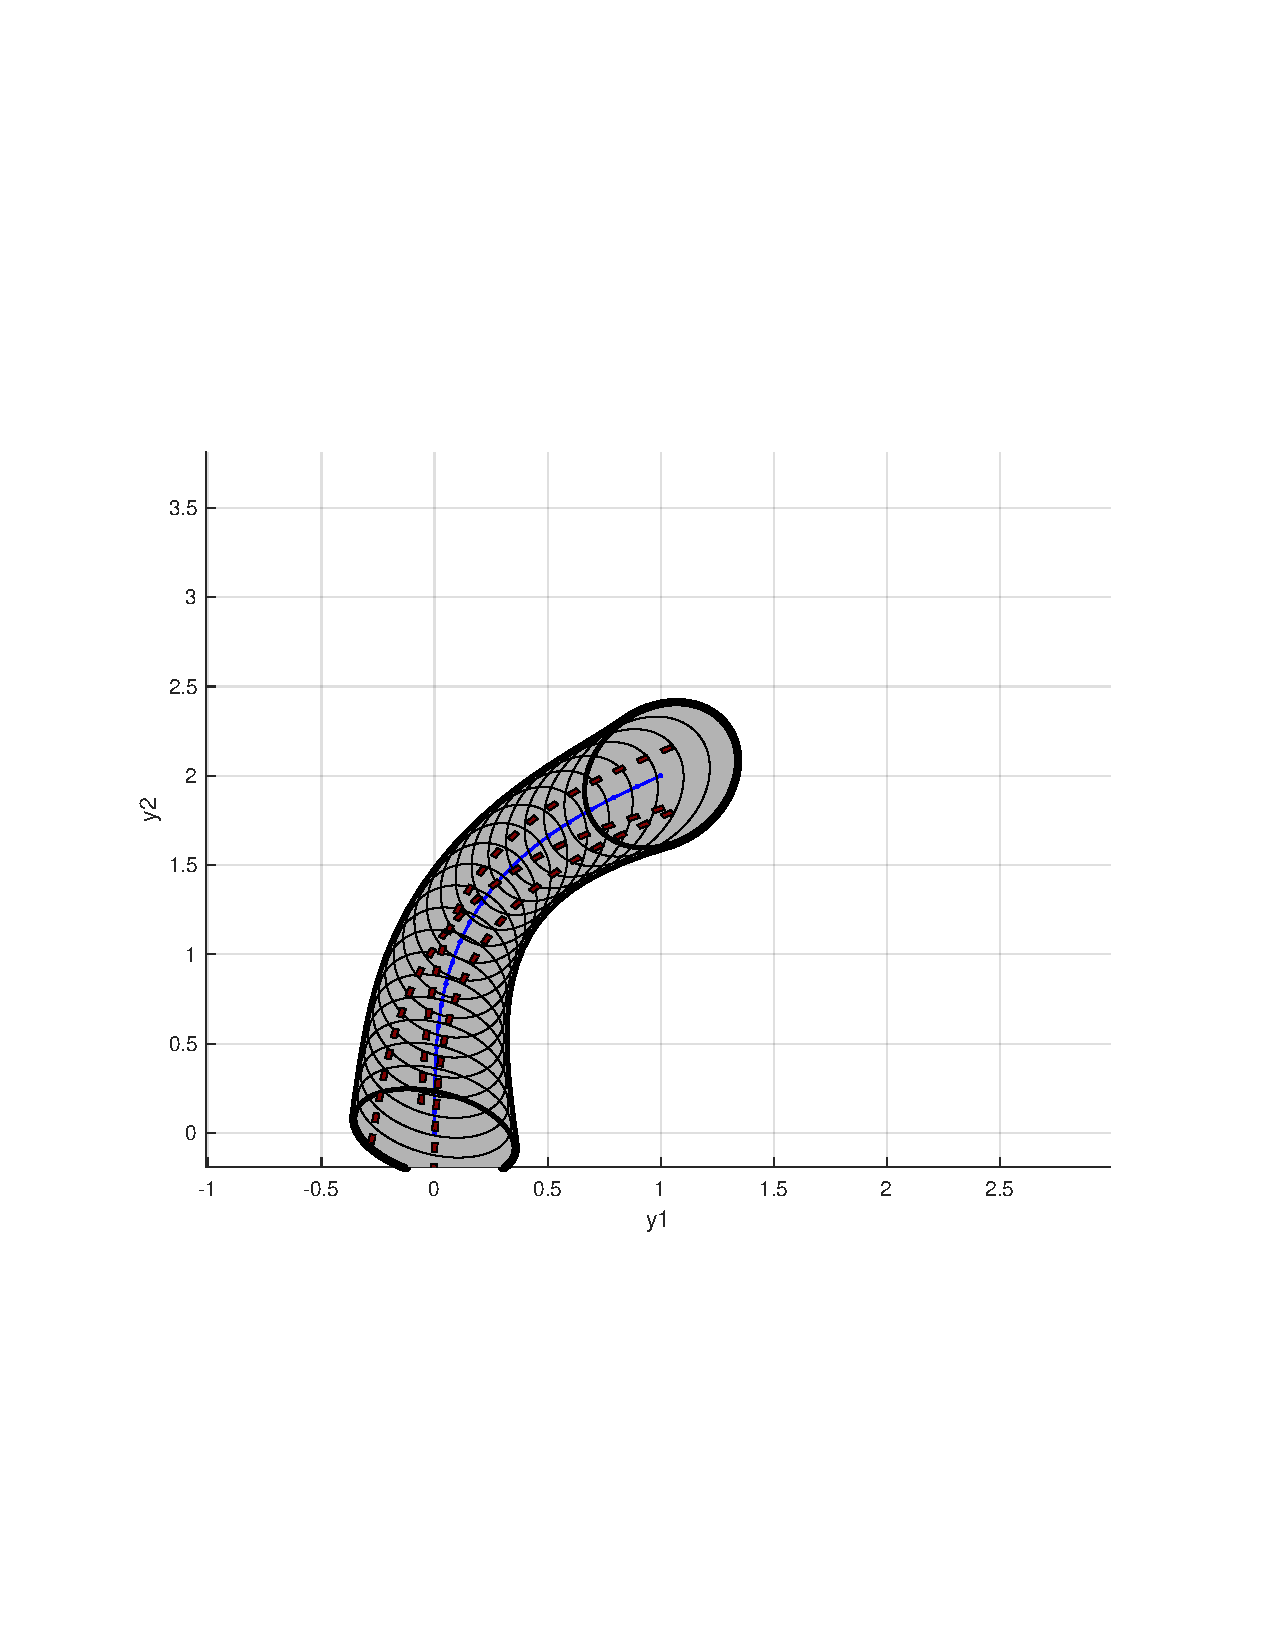
\includegraphics[scale=0.5]{figures/funnel/right_simulation}
  \caption{Three simulations of the right funnel with different initial
    conditions, where two out of three funnels left the inside of the funnel.
    Right now I can only speculate as to why this is happening.}
\end{figure}

For the model with uncertainty added to the speed of the vehicle, we get:

\subsection{Only minimizing the volume of the funnel projected down into the
  xy-plane}

There is no need in minimizing the value of \(\dot{\theta}\), so in order to
minimize what we care about, i.e. the actual size of the funnel where the
physical vehicle can move, we modify our costfunction according to
\cite{majumdarFunnelLibrariesRealtime2017}. Thus, given a projection map \(\pi :
\R^n \rightarrow \R^{n_p}\). Given the ellipsoid \(\epsilon = \set{\bar{x} \in
  \R^n | \bar{x}^TS_{k}\bar{x} \leq 1}\) with
\[
  \S_k^{(p)} = (\p{PS_k^{-1}P^T}^{-1})
\]
Given that minimizing the volume of the ellipsoid \(\epsilon\) using an SDP
relies on maximizing the determinant of \(S_k\). Since \(det(S_k)\) is a
nonlinear function of \(S_k\), the function has to be linearized in order for it
to be handled by our solution framework (SOS-programming).
\cite{majumdarFunnelLibrariesRealtime2017} solves this by linearizing
\(det(S_k)\) at the solution of \(S_k\) from the previous iteration, and
maximizes this linearization instead. In the end this translates to
\[
  lin\p{det\p{S_k}} =
  Tr\p{P^T\p{PS_{k,0}^{-1}P^T}^{-1}PS_{k,0}^{-1}S_kS_{k,0}^{-1}}
\]
where \(S_{k,0}\) is the nominal value.

\subsection{Checking composability of Funnels}

In order for two \funnel's to be composable, the outlet of one \funnel\ needs to
be completely contained within the inlet of the other. This means that if
\(\mathcal{F}_1 = F_1(T)\) is the outlet of \funnel\ \(F_1\), and
\(\mathcal{F}_2 = F_2(0)\) is the inlet of \(F_2\), then
\[
  \mathcal{F}_1 \subseteq \mathcal{F}_2
\]
in order for the funnels to be composable. In this thesis this composition
checking is done off-line and prior to the algorithms run. First however, how to
verify that the outlet of one \funnel\ is fully contained within the inlet of
the other.

In \cite[Majumdar and Tedrake, p.~47]{majumdarFunnelLibrariesRealtime2017}, two
funnels are sequentially composable if
\begin{definition}
  An ordered pair \((F1, F2)\) of funnels \(F_1 \colon [0,T_1] \rightarrow
  \mathcal{P}(\R^n)\) and \(F_2 \colon [0,T_2] \rightarrow \mathcal{P}(\R^n)\)
  is sequentially composable if \(F_1(T) \subseteq F_2(0)\).
\end{definition}

TODO - make pretty funnel picture!

\subsection{Shifting funnels around in the world frame}
